\section{Event Types}

To measure the hadronic $\Upsilon$ cross-section at each energy point,
I must count the number of hadronic $\Upsilon$ decays, and divide by a
count of selected gamgams or bhabhas (then make a correction for beam
energy).  To do so, I will need selection criteria (from here on, also
known as ``cuts'') for identifying a given event as a hadronic
$\Upsilon$ decay, and another set of criteria for identifying a gamgam
or a bhabha.

Not every event that passes cuts is a real $\Upsilon$ decay, but the
majority of these ``backgrounds'' can be eliminated by subtracting a
sample that contains only backgrounds.  The off-resonance data is such
a sample: they contain no $\Upsilon$ decays and all background event
types, but not necessarily in the right proportion.  All products of
$e^+e^-$ interactions are in proportion to the number of $e^+e^-$
collisions, so these backgrounds ``scale with'' the integrated
luminosity of each run.  But three backgrounds are not products of
$e^+e^-$ interactions: beam-gas, beam-wall, and cosmic rays.

Beam-gas and beam-wall collisions, where an electron or positron from
one beam collides with a gas atom or the wall of the beam pipe, scale
with the individual beam currents (which can be different) and the air
pressure inside the beam pipe.  To track this background on a
run-by-run basis (and to make sure it never gets too large), I
additionally defined cuts for beam-gas events, and distinguish between
positron beam-gas and electron beam-gas to indirectly measure the two
beam currents independently.  (Beam-gas is a sub-percent background
after hadron cuts and continuum subtraction, and beam-wall is much
smaller, so I will assume that the beam-wall count scales
proportionally with the beam-gas count for each beam.)

Cosmic rays scale with time and are completely independent of the
instantaneous luminosity.  I track these the same way as electron and
positron beam-gas: by defining an event type and counting them.

A different way hadronic $\Upsilon$ counting can fail is if either the
DR or the CC loses sensitivity (e.g. by losing high voltage) and the
other doesn't.  For some fraction of a run, I would lose sensitivity
to hadrons but not to gamgams (or vice-versa) and get a hadronic
cross-section which is too small (or too large).  To check for DR
failures, I select bhabhas using only CC criteria and ask how many of
them have no tracks: ``trackless bhabhas.''  To check for CC failures,
I compare the bhabha count with a mupair count, which differs only in
that bhabhas deposit a lot of energy in the CC and mupairs deposit
very little.  If the CC were to fail while the DR continued to take
data, the huge bhabha count would drop to zero and the mupair count
would surge unbelievably high.  Even though mupairs interfere more
than bhabhas with the $\Upsilon$ resonance, we are looking for much
more dramatic variations in the bhabha/mupair ratio.  The events used
for this purpose must have a DR-only trigger, so they are called
DR-trigger bhabhas and DR-trigger mupairs.  These three event types,
trackless bhabhas, DR-trigger bhabhas and DR-trigger mupairs, will be
counted not only run-by-run, but for each hundredth part of a run, so
that an instrumental failure can be more easily recognized.

These nine event types are defined in Table \ref{cuts:eventtypes}.
For simplicity, they have been defined to be mutually exclusive
(except for bhabhas and DR-trigger bhabhas).

\section{Variables}

Every cut will be defined in terms of one of the following variables.

\subsection{Trigger Decision and \lfourdec}

For an event to be fully read out of the CLEO detector, let alone
saved to disk, it must pass one of the hardware triggers.  These
triggers are therefore the first cuts to be applied to data.  The
trigger lines which are relevant for my event types are: Hadron,
RadTau, ElTrack, BarrelBhabha, and TwoTrack.

All of these trigger lines are logical combinations of a minimum
number of AXIAL tracks, STEREO tracks, and CBLO, CBMD, and CBHI
clusters, which I will define shortly.  The algorithm for each trigger
decision is presented in Table \ref{cuts_triggerlines}.

An AXIAL track is a connected sequence of DR hits with at least 6 hits
in the first 8 layers of the DR and at least 6 hits in the next 8
layers of the DR.  A STEREO track is an extension of an AXIAL track
into the remaining 31 layers, so the number of STEREO tracks is always
less than or equal to the number of AXIAL tracks.

For the purposes of the trigger, the CC barrel is divided into 16
sections in $\phi$ by 12 in Z, called tiles.  If the total energy in a
tile is greater than 0.15 GeV, it counts as a CBLO cluster, if the
energy is greater than 0.75 GeV, it is also a CBMD, and if the energy
is greater than 1.5 GeV, it is also a CBHI.  (\#CBLO $\ge$ \#CBMD
$\ge$ \#CBHI.)  The division of the CC barrel into tiles introduces an
edge effect: a high-energy shower can deposit energy into several
adjacent tiles, in which none of them satisfy a given threshold,
though the whole shower would have.  This makes the cluster efficiency
asymmetric around its threshold energy, as seen in Figure
\ref{trigger_topher}.

\begin{table}[p]
  \caption{\label{cuts_triggerlines} Definition of each trigger line
    in terms of low-level trigger variables}
  \begin{center}
    \begin{tabular}{r p{0.7\linewidth}}
      Hadron & \#AXIAL $\ge$ 3 and \#CBLO $\ge$ 1 \\
      RadTau & \#STEREO $\ge$ 2 and (\#CBLO $\ge$ 2 or \#CBMD $\ge$ 1) \\
      ElTrack & \#AXIAL $\ge$ 1 and \#CBMD $\ge$ 1 \\
      BarrelBhabha & \#CBHI in east $\ge$ 1 and \#CBHI in west $\ge$ 1
      (with very weak back-to-back requirements in $\phi$)\\
      TwoTrack & \#AXIAL $\ge$ 2 with a prescale
    \end{tabular}
  \end{center}
\end{table}

\begin{figure}[p]
  \begin{center}
    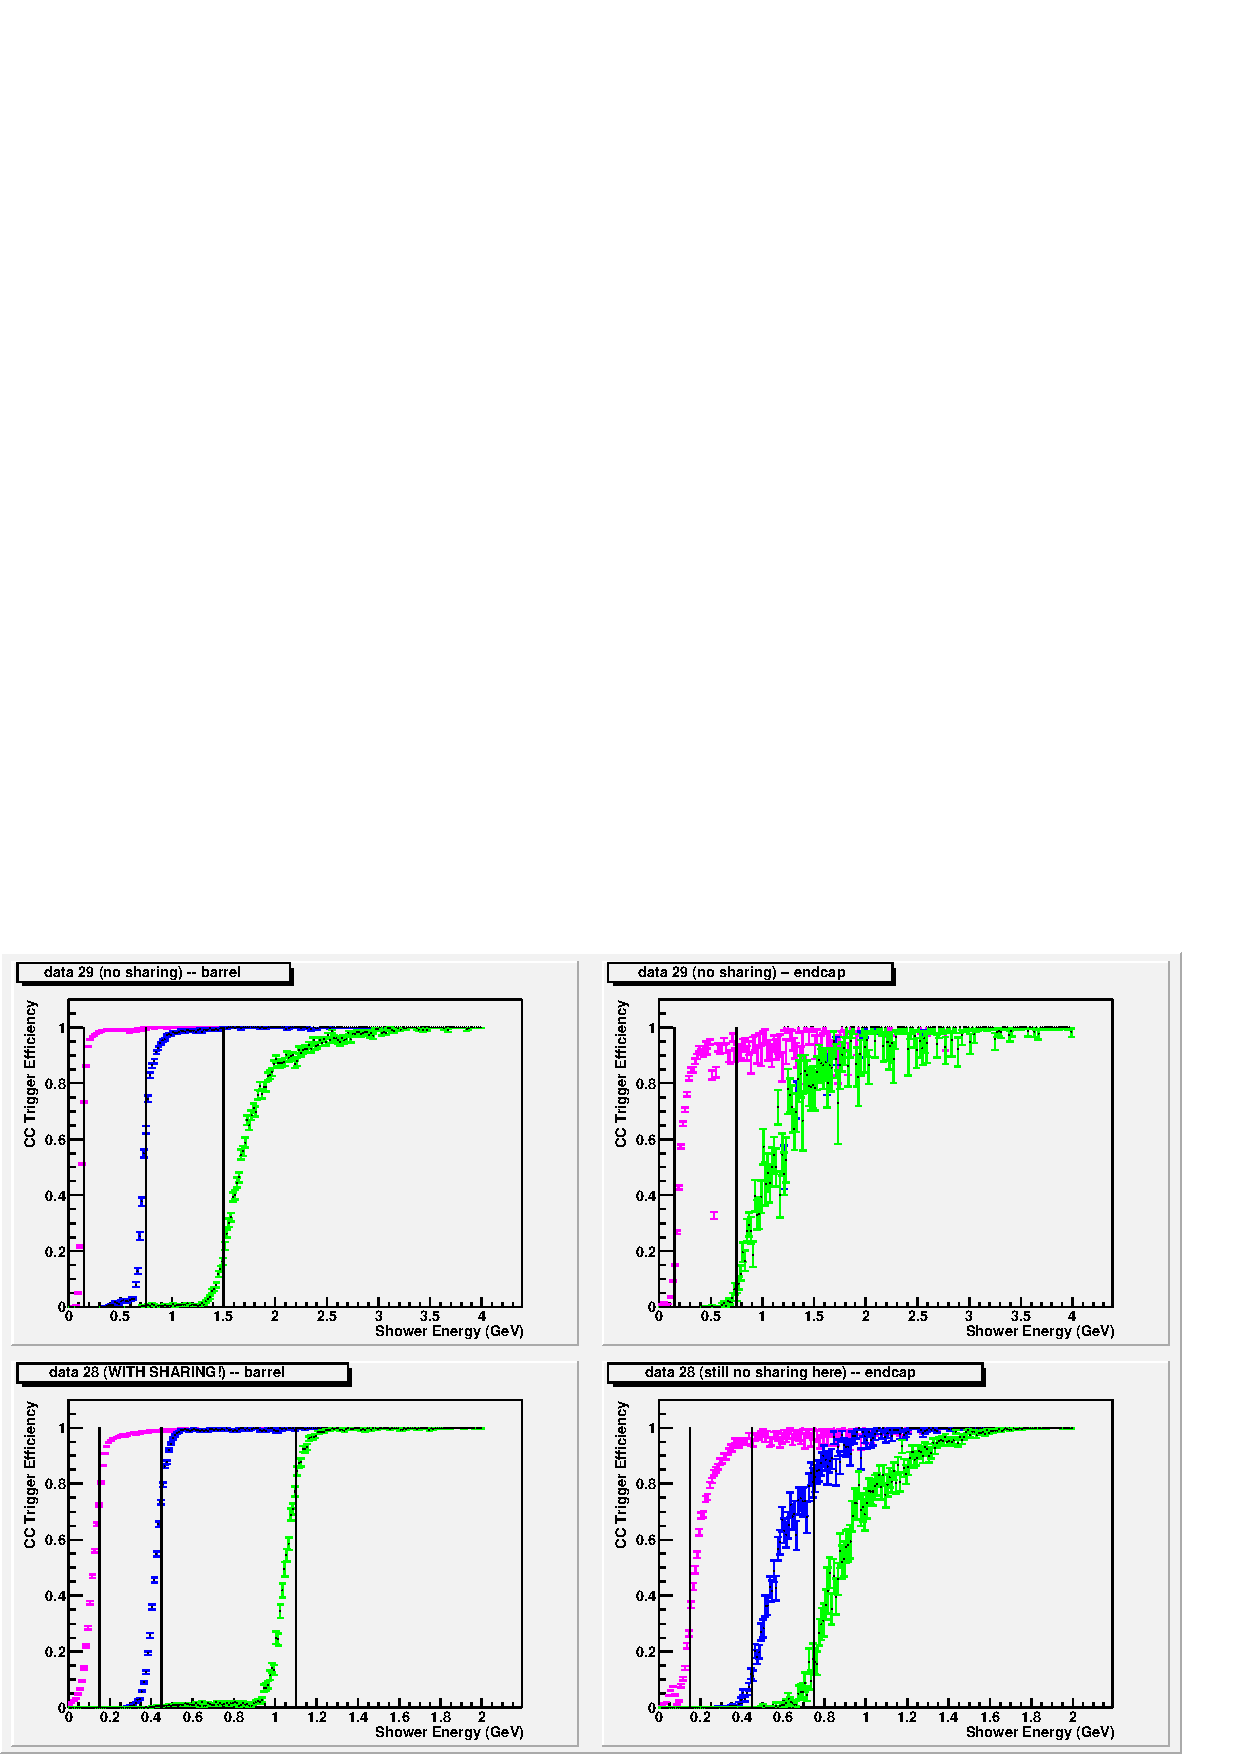
\includegraphics[width=\linewidth, clip=true]{plots/trigger_topher}
  \end{center}
  \caption{\label{trigger_topher} Cluster energy thresholds for CBLO
  (0.15 GeV), CBMD (0.75 GeV), and CBHI (1.5 GeV) (left to right), as
  measured in data with isolated showers.}
\end{figure}

The BarrelBhabha trigger line is the only one which relies entirely on
the CC, making it appropriate for gamgam counting.  In addition to
demanding two CBHI clusters, it requires them to be in opposite halves
of the detector, which introduces an edge effect (low efficiency) near
$\cos\theta$ = 0.  The TwoTrack trigger line relies entirely on the
DR, but it is prescaled by a factor of 19 (18 out of 19 events with
two AXIAL tracks are fail this trigger line), making it useful only as
a diagnostic.

All data in the CLEO-III database was additionally passed through a
software filter called level 4.  The algorithm which processes this
decision (\lfourdec) is complicated, but it can be bypassed by
re-processing raw data.  It is extremely loose for $\Upsilon$ events,
especially after all other cuts.

\subsection{Displacement of the Primary Vertex (\dxy\ and \dz)}

The location of the primary vertex is represented by two variables.
In XY (the plane of the DR), the closest approach of the closest track
to the beam spot is labeled \dxy.  Hadronic events with many tracks
and bhabhas/mupairs with very precise tracks usually have a \dxy\ below
1 mm, but I cut at 5 mm, just in case the reported beam spot is wrong
by a few millimeters.  The beam spot is the average primary vertex for
each run, determined by vertex-fitting the first 500 hadronic events
of that run.

I determine the Z position of the primary vertex (\dz) with a more
complicated algorithm.  When projected into the XY plane, each track
traces a directed circle, and every pair of circles intersects at
zero, one, or two points.  For each pair of tracks that intersects in
XY, I choose the intersection point which is closest to the beam spot
(in the forward direction of the particle's trajectory), and calculate
the weighted mean of their Z positions.  (The Z of an intersection is
the average Z, $(Z_1 + Z_2)/2$, at the point of intersection.)  The
``errors'' used in the weighted average are
\begin{equation}
  \sqrt{{\sigma_{\mbox{\scriptsize intersection}}}^2 + (\mbox{separation in
      Z})^2 + (\mbox{XY distance from the beam spot})^2}
\end{equation}
where $\sigma_{\mbox{\scriptsize intersection}}$ is the uncertainty in
the Z of each intersection point (from track fitting), and the
``separation in Z'' and ``XY distance from the beam spot'' are both
calculated at the intersection point.  With this assumed error, not
only are badly-fit tracks deweighted, but also tracks which don't come
close to intersecting in all three dimensions, and intersections that
don't seem to come from the primary vertex.  As a result, this average
of intersections characterizes the primary vertex location well, and
compares favorably with a $\chi^2$-based vertex fitter.  This method
is preferred because the $\chi^2$ fitter fails on too many events to
effectively identify beam-gas.  The average of intersections will only
fail to return a result if there are fewer than two tracks which reach
the stereo layers of the DR, or if no tracks overlap in the forward
directions.  If it does exist, \dz\ is this average of intersections.
If not, it is the closest approach of the closest track to the beam
spot in Z (by analogy to \dxy).  This combined method only needs one
track in the DR.  Like \dxy, I cut far from the bulk of the
distributions (which are about 2 cm wide), at 7.5 cm.

\subsection{Quality Tracks and Quality Showers}

The tracks used to define \dxy\ and \dz\ are unconstrained: any track
which was identified by pattern recognition is used.  Other quantities
such as the number of tracks and the visible energy will draw on a
more restricted set of tracks, called ``quality'' tracks, which
satisfy the following criteria.
\begin{itemize}
  \item The track fitter (Kalman algorithm) must not fail.

  \item Track $\chi^2$ $/$ \#degrees of freedom $<$ 100, with $>$ 0
    degrees of freedom.

  \item Expected \#layers hit $/$ \#layers actually hit must be
    between 0.5 and 1.2.  (Two hits in the same DR layer count as one
    layer hit.)

  \item \label{cuts:trackd0z0} Closest approach to the DR origin
    (which is always within a centimeter of the beam spot) $<$ 3 cm in
    XY and 18 cm in Z.

  \item Momentum must be between 1\% and 150\% \ebeam.

  \item Track $|\cos\theta|$ $<$ 0.95.

  \item Fitting uncertainties in $\cot\theta$ and $z_0$ are less than
    0.50 and 25 cm, respectively.
\end{itemize}
Quality showers must pass this set of cuts:
\begin{itemize}
  \item Shower energy $>$ 1\% \ebeam.

  \item The shower ``status'' is true, and

  \item the shower is not identified as being ``hot.''
\end{itemize}
Hot (or noisy) showers are recognized by their high output over small
ranges of run numbers.

When tracks or showers are not specified as ``quality,'' all tracks or
showers are intended.

\subsection{Biggest Track Momenta (\pone, \ptwo) and Biggest Shower
  Energies (\eone, \etwo)}

The biggest track momentum variables \pone\ and \ptwo\ and the biggest
shower energy variables \eone\ and \etwo\ are taken from the set of
quality tracks and quality showers.  If not enough quality tracks or
quality showers are present, they default to zero (and therefore pass
upper limits and fail lower limits).

\subsection{Visible energy (\visen)}

The visible energy, or \visen, is the sum of all charged energy and
neutral energy in an event.  The charged energy is the sum of all
quality track energies, assuming their masses to be $m_\pi$ = 140 MeV.
If any track is an electron (matched to a shower with $E/p$ $>$ 0.5),
the sum also includes all associated bremsstrahlung showers (over 1\%
\ebeam).  The neutral energy is the energy sum of all quality showers
for which:
\begin{itemize}
  \item standard track-shower matching failed,

  \item track-shower matching using connected regions failed, and

  \item the shower is not identified as bremsstrahlung for an electron
    ($E/p$ $>$ 0.5).
\end{itemize}

Note that a particle can fail to be identified as charged or neutral
if it leaves a non-quality track which is matched to a shower.  The
track-shower matching will disqualify the shower as neutral energy,
and the fact that the track failed quality cuts will disqualify it as
charged energy.  Many cosmic rays are calculated as having zero
\visen\ because the tracks are more than 3 cm from the DR origin and
the two muon showers in the CC are matched to tracks.

Sometimes I will need to refer to an event's hot visible energy,
\hotvisen, which is calculated the same way except that hot crystals
are not ignored.  Note that \hotvisen\ $\ge$ \visen, so if an event
has \visen\ $>$ some threshold, it will automatically have \hotvisen\
$>$ that threshold.

\subsection{Initial-State Radiation for Bhabhas/Mupairs (\eisr)}

Bhabhas and mupairs can be identified by two high-momentum tracks, but
greater precision can be obtained by additionally constraining the
4-momentum of the largest radiated photon.  Given a reconstructed
bhabha/mupair event, the momentum of all associated photons is
\begin{equation}
  E_{\mbox{\scriptsize ISR}} = \vec{p}_1 + \vec{p}_2 - \vec{\alpha}
\end{equation}
where $\vec{p}_1$ and $\vec{p}_2$ are the two largest track momenta
and $\vec{\alpha}$ is the sum of the incident beam momenta in the lab
frame.  This $\vec{\alpha}$ is exactly zero in the Monte Carlo and
very close to zero in data: 25 MeV toward the center of the storage
ring, due to a small crossing angle of the two beams.

When one photon dominates the neutral energy in a bhabha/mupair event,
\eisr\ is approximately the momentum, and therefore the energy, of
that photon.  (It is usually also an initial state photon, pointing
along the beam line.)  In that case, \ecom\ $-$ \pone\ $-$ \ptwo\ $-$
\eisr\ is zero, or close to it, by energy conservation.  (The center
of mass energy, \ecom, is defined to be twice the beam energy, with no
attempt to correct for crossing angle.)

\subsection{Two-Track Back-to-Backness (\pdotp)}

More back-to-back than bhabhas and mupairs, which radiate at the
primary vertex, are the two tracks associated with a single cosmic
ray.  The fact that a single cosmic ray is identified as having two
tracks is an artifact of track-finding: the pattern recognition
expects particles to originate near the DR origin.  The cosine of the
angle between these two tracks, $\vec{p}_1\cdot\vec{p}_2$, differs
from 1 or -1 by no more than tracking resolution, which is typically
in the fifth digit.  The two vectors used in the dot product are the
two largest quality track momenta, $\vec{p}_1$ and $\vec{p}_2$,
evaluated at the closest point to the DR origin (which will be the
same point for cosmic ray tracks).

\subsection{Net Z momentum (\pz)}

Electron beam-gas and positron beam-gas are distinguished from one
another by the sum of the Z momenta of all tracks in the event (not
just quality tracks).  Gas atoms in the beam pipe are essentially at
rest, so the final state momentum of the system cleanly tags the
incident particle as a westward-going positron (positive \pz) or an
eastward-going electron (negative \pz).

\section{Event Selection}

In addition to the hardware trigger and \lfourdec, events were
filtered before being stored in the CLEO-III database.  These
selection criteria are complicated, but the following sufficient
conditions for appearing in the database include nearly all of the
interesting events.
\begin{itemize}
  \item An event is in the CLEO-III database if \hotvisen\ $>$ 40\%
    \ecom.

  \item \label{wonderfuldiscovery} An event is in the CLEO-III
    database if \hotvisen\ $>$ 4\% \ecom\ and the event has two or
    more quality tracks.
\end{itemize}

Just as with \lfourdec, these pre-selection criteria can be bypassed
by extracting raw data.  This will be discussed further in the next
chapter.  But in the interest of saving processing time and
duplication of effort, my event selection criteria should be subsets
of the above.  This is only limiting when I want to extract cosmic
rays or beam-gas, which are usually not desirable for physics.

The efficiency of the hadron cuts will need to be very well
understood, so they should be simple and loose.  I have also given
them an ordering, so that each cut can be studied with all previous
cuts applied, and no assumptions will need to be made about their
correlations.  They will be studied using raw data, so \visen\ and
\lfourdec\ can be applied last.  The trigger, of course, must be
applied first.  These cuts are listed first in Table
\ref{cuts:eventtypes}.

\begin{figure}[t]
  \begin{center}
    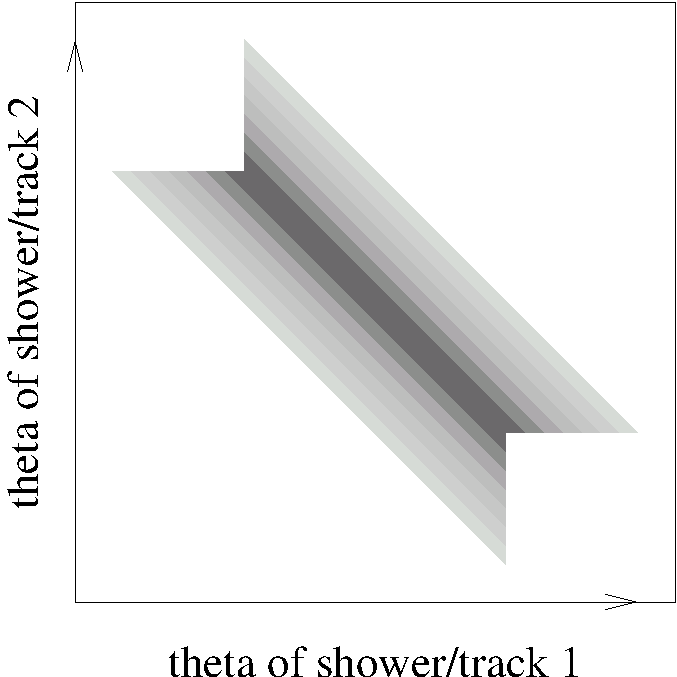
\includegraphics[width=0.4\linewidth]{plots/explain_asymmetric_cut}
  \end{center}
  \caption{\label{cuts:explain_asymmetric_cut} A cartoon of the
    geometry of an asymmetric cut for two anti-correlated showers or
    tracks.  Dark gray corresponds to a high event population, and the
    light gray smearing on both sides of the distribution represents
    effects of initial and/or final state radiation, and measurement
    error.  The purpose is to place an upper limit on $\theta$ that
    minimally depends on radiation and measurement error.}
\end{figure}

Cuts for gamgams and bhabhas include asymmetric upper limits on
$|\cos\theta|$, as depicted in Figure \ref{cuts:explain_asymmetric_cut}.
These ensure that no hard cut is made in the middle of a two-particle
angular distribution.  Gamgam selection criteria also include an
asymmetric lower limit on $|\cos\theta|$ and three rejected
$\theta-\phi$ regions.  These cover holes in the BarrelBhabha trigger
efficiency that are either hard to predict (edge effect near
$|\cos\theta|$ = 0) or vary from run to run (missing tiles in the
trigger and a wire mis-map).  Also, gamgam cuts are defined in terms of
$\cot\theta$ rather than $\cos\theta$ because their efficiency depends
on a crystal granularity that is periodic in $\cot\theta$.  High
\hotvisen\ is guaranteed by putting lower limits on \ptwo\ and \etwo.

Trackless bhabha cuts are a copy of the gamgam cuts, with a different
$\phi$ back-to-backness criterion to allow the electrons to bend in
the magnetic field.  Also, the no-track criterion is tightened,
refusing even trigger tracks.  Technically, this is achieved by
requiring the ElTrack trigger line to fail.  ElTrack requires a
trigger track and a CC cluster which is already guaranteed by the
BarrelBhabha trigger.  Therefore, if ElTrack fails, no trigger track
was found.

DR-trigger bhabhas differ only from ordinary bhabhas in relying on the
TwoTrack trigger rather than the union of Hadron, RadTau, and ElTrack.
This is for the purpose of being independent of the CC.  The same is
true of DR-trigger mupairs, except that mupairs cannot have more than
1 GeV of CC energy (consistent with two minimum-ionizing particles or
a loss of CC signal).

For beam-gas and cosmic rays, I take advantage of the second
sufficient condition on page \pageref{wonderfuldiscovery} to obtain
events with very low \hotvisen: I require two quality tracks.  This
isn't optimally efficient, as beam-gas tracks often fail the quality
cuts, and cosmic rays beyond 3 cm of the DR origin (most of them) must
fail.  (The database event filters were not designed to save beam-gas
events and cosmic rays!)  The geometric variables \dxy\ and \dz\ are
used to distinguish the two types from each other and from beam-beam
interactions because beam-gas events can happen anywhere along the
beam line, and cosmic rays usually miss the beam line.  Additional
cosmic ray/beam-gas discrimination comes from \pdotp.

All cuts are listed in Table \ref{cuts:eventtypes}.

\begin{table}[p]
  \caption{\label{cuts:eventtypes} All event types and corresponding
    selection criteria used in this analysis}

  \vspace{0.5 cm}
  \noindent \begin{tabular}{p{0.24\linewidth} p{0.70\linewidth}}
    Event type & Event selection criteria \\\hline
  \end{tabular}
  \vspace{-1 cm}
\end{table}

\begin{table}[p]
  \noindent \begin{tabular}{p{0.24\linewidth} p{0.70\linewidth}}
    hadron & 1. Hadron, RadTau, or ElTrack trigger line \\
    	   & 2. closest track to beam spot in XY (\dxy) $<$ 5 mm \\
    	   & 3. Z of primary vertex (\dz) within 7.5 cm of beam spot \\
    	   & 4. biggest-momentum track (\pone) $<$ 80\% \ebeam \\
    	   & 5. visible energy (\visen) $>$ 40\% \ecom \\
    	   & 6. passes software level 4 decision (\lfourdec) \\
  \end{tabular}
\end{table}

\begin{table}[p]
  \noindent \begin{tabular}{p{0.24\linewidth} p{0.70\linewidth}}
    gamgam & BarrelBhabha trigger line and \lfourdec \\
           & two biggest-energy showers are on opposite sides of CC \\
           & second-biggest energy shower (\etwo) $>$ 70\% \ebeam \\
           & zero quality tracks \\
           & $|\cot\theta_1 + \cot\theta_2|$ $<$ 0.1 (showers back-to-
             back in $\theta$) \\
           & $|\sin(\phi_1 - \phi_2)|$ $<$ 0.04 (showers back-to-back
             in $\phi$) \\
           & ($|\cot\theta_1|$ $<$ 1.28 and $|\cot\theta_2|$ $<$ 1.18) \\
           & \mbox{\hspace{0.5 cm}} or ($|\cot\theta_1|$ $<$ 1.18 and
	     $|\cot\theta_2|$ $<$ 1.28) (in CC barrel) \\
           & ($|\cot\theta_1|$ $>$ 0.05 and $|\cot\theta_2|$ $>$ 0.15) \\
           & \mbox{\hspace{0.5 cm}} or ($|\cot\theta_1|$ $>$ 0.15 and
	     $|\cot\theta_2|$ $>$ 0.05) \\
	   & reject ($-\frac{14}{64}\pi$ $<$ $\phi_{\mbox{\scriptsize
             west}}$ $<$ $\frac{9}{64}\pi$ and average $|\cot\theta|$
             $<$ 0.54) \\
	   & reject ($-\frac{53}{64}\pi$ $<$ $\phi_{\mbox{\scriptsize
             west}}$ $<$ $-\frac{14}{64}\pi$ and average $|\cot\theta|$
             $>$ 0.95) \\
	   & reject ($-0.4$ $<$ $\phi_{\mbox{\scriptsize west}}$ $<$
             $-0.3$) \\
  \end{tabular}
\end{table}

\begin{table}[p]
  \noindent \begin{tabular}{p{0.24\linewidth} p{0.70\linewidth}}
    trackless bhabha & same as gamgam except 0.04 $<$ $|\sin(\phi_1 -
                       \phi_2)|$ $<$ 0.25 \\
		     & \mbox{\hspace{0.5 cm}} and NO tracks are
                       allowed, not even trigger tracks \\
  \end{tabular}
\end{table}

\begin{table}[p]
  \noindent \begin{tabular}{p{0.24\linewidth} p{0.70\linewidth}}
    bhabha & hadron's trigger lines, \lfourdec, \dxy, and \dz\ constraints \\
           & two biggest-momentum tracks have opposite charges \\
           & second-biggest momentum track (\ptwo) $>$ 70\% \ebeam \\
	   & ($|\cos\theta_1|$ $<$ 0.79 and $|\cos\theta_2|$ $<$ 0.76) \\
	   & \mbox{\hspace{0.5 cm}} or ($|\cos\theta_1|$ $<$ 0.76 and
             $|\cos\theta_2|$ $<$ 0.79) \\
	   & \eisr\ $<$ 20\% \ebeam \\
	   & \ecom\ $-$ \pone\ $-$ \ptwo\ $-$ \eisr\ $<$ 20\% \ecom \\
	   & second-biggest energy shower (\etwo) $>$ 40\% \ebeam
  \end{tabular}
\end{table}

\begin{table}[p]
  \noindent \begin{tabular}{p{0.24\linewidth} p{0.70\linewidth}}
    DR-trigger bhabha & same as bhabha except TwoTrack trigger only \\
  \end{tabular}
\end{table}

\begin{table}[p]
  \noindent \begin{tabular}{p{0.24\linewidth} p{0.70\linewidth}}
    DR-trigger mupair & same as DR-trigger bhabha except \\
                      & \mbox{\hspace{0.5 cm}} second-biggest energy
                        shower (\etwo) $<$ 1 GeV \\
  \end{tabular}
\end{table}

\begin{table}[p]
  \noindent \begin{tabular}{p{0.24\linewidth} p{0.70\linewidth}}
    electron beam-gas & hadron's trigger lines, \lfourdec, and \dxy\
                        constraints \\
                      & Z of primary vertex (\dz) $>$ 7.5 cm \\
                      & $\ge$ 2 quality tracks and \visen\ $>$ 4\% \ecom \\
                      & two-track back-to-backness (\pdotp) $<$ 0.9 \\
                      & net Z momentum (\pz) $<$ $-$0.1 \ebeam\ (east) \\
  \end{tabular}
\end{table}

\begin{table}[p]
  \noindent \begin{tabular}{p{0.24\linewidth} p{0.70\linewidth}}
    positron beam-gas & same as electron beam-gas except \\
                      & \mbox{\hspace{0.5 cm}} net Z momentum (\pz)
                        $>$ $+$0.1 \ebeam\ (west) \\
  \end{tabular}
\end{table}

\begin{table}[p]
  \noindent \begin{tabular}{p{0.24\linewidth} p{0.70\linewidth}}
    cosmic ray & hadron's trigger lines and \lfourdec \\
               & closest track to beam spot in XY (\dxy) $>$ 5 mm \\
               & $\ge$ 2 quality tracks and \visen\ $>$ 4\% \ecom \\
               & two-track back-to-backness (\pdotp) $>$ 0.999 \\
               & total CC energy $<$ 2 GeV \\
  \end{tabular}
\end{table}


